\chapter{Simulation results}\label{ch:simulationResults}
\noindent This chapter summarizes defines \textit{Virtual playground} where MPC approach was tested. Other sections summarizes simulation results, taking into account: obstacle avoidance (safety margin), control quality (prediction deviation).
\section{Playground definition}\label{ch:3DPlaygroundDefinition}
\noindent For purpose of new theorem formulation, new playground (\ref{fig:new3DPlayground})with added dimension needs to be introduced. Additional element of \textit{mission control} needs to be introduced, because previous experiments was with not coordinated flight and for real missions some coordinated flight is required, therefore waypoint set $\mathscr{WP}$ is added into playground. 
\begin{figure}[H]
    \centering
    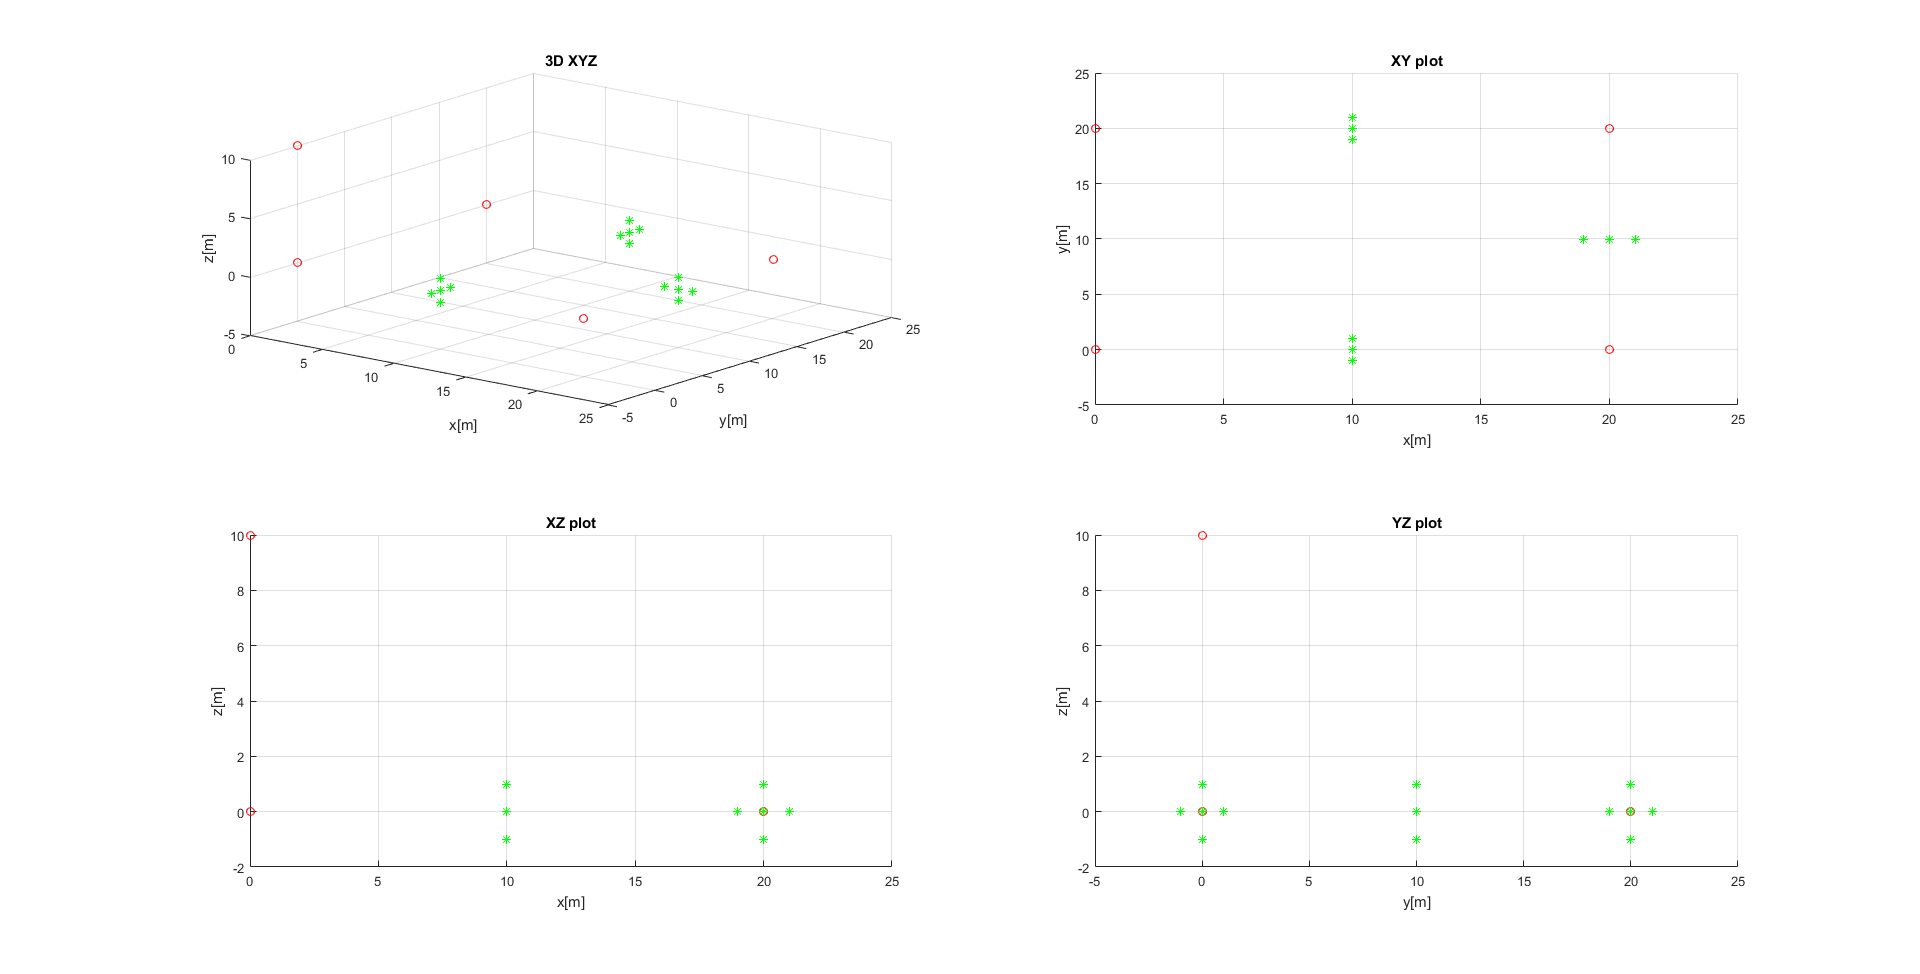
\includegraphics[width=\linewidth]{\FIGDIR/37_Playground_3D.png}
    \caption{Initial playground for obstacle avoidance and optimal path finding testing}
    \label{fig:new3DPlayground}
\end{figure}
\newpage\noindent Waypoint set $\mathscr{WP}$ (\ref{eq:playground3DSimpleWPSet}) contains five waypoins in Cartesian coordinates $\mathscr{WP}_i =[x,y,z]^T$. This set is simple rectangular flight around rectangle with side of 20 meters and slightly elevated end by 10 meters $\mathscr{WP}_E$.

\begin{equation}\label{eq:playground3DSimpleWPSet}
    \begin{aligned}
          \mathscr{WP} = \{ \mathscr{WP}_S &=[0,0,0]^T,\\
                            \mathscr{WP}_1 &=[20,0,0]^T,
                            \mathscr{WP}_2 =[20,20,0]^T,\\
                            \mathscr{WP}_3 &=[0,20,0]^T,
                            \mathscr{WP}_E =[0,0,10]^T,\}
    \end{aligned}
\end{equation}
\noindent Each path tracking algorithm needs to have stop condition which indicates when vehicle should stop following presented waypoint. Usually unit ball stop condition is used (\ref{eq:stopFunctionUnitBall}) where $[x_v,y_v,z_v]^t$ is vehicle position, $[x_g,y_g,z_g]^T$ is waypoint position and $p_t$ is precision threshold.
\begin{equation}\label{eq:stopFunctionUnitBall}
    \norm{\begin{bmatrix}x_g-x_v\\y_g-y_v\\z_g-z_v\end{bmatrix}} \le p_t
\end{equation}
Complete obstacle definition with associated structure can be found in section \ref{s:3dObstacleRepresentationSimplistic}. Single obstacle $o_i\in\mathscr{O}$ is defined by its position $o=[x_o,y_o,z_o]^T$. All obstacles are stored in single obstacle structure $\mathscr{O}$ defined by (\ref{eq:3dSimplisticPlaygroundO}).
\begin{equation}\label{eq:3dSimplisticPlaygroundO}
    \mathscr{O} = \{\mathscr{O}_1,\mathscr{O}_2,\mathscr{O}_3\}
\end{equation}
Obstacle subset $\mathscr{O}_1$ (\ref{eq:3dSimplisticPlaygroundO1}) is defined between waypoints $\mathscr{WP}_S,\mathscr{WP}_1$.
\begin{equation}\label{eq:3dSimplisticPlaygroundO1}
    \mathscr{O}_1 = \{[10,0,0]^T,[10,1,0]^T,[10,-1,0]^T,[10,0,1]^T,[10,0,-1]^T\}
\end{equation}
Obstacle subset $\mathscr{O}_2$ (\ref{eq:3dSimplisticPlaygroundO2}) is defined between waypoints $\mathscr{WP}_1,\mathscr{WP}_2$.
\begin{equation}\label{eq:3dSimplisticPlaygroundO2}
    \mathscr{O}_2 = \{[20,10,0]^T,[20,10,1]^T,[20,10,-1]^T,[19,10,0]^T,[21,10,0]^T\}
\end{equation}
Obstacle subset $\mathscr{O}_3$ (\ref{eq:3dSimplisticPlaygroundO3}) is defined between waypoints $\mathscr{WP}_2,\mathscr{WP}_3$.
\begin{equation}\label{eq:3dSimplisticPlaygroundO3}
    \mathscr{O}_3 = \{[10,20,0]^T,[10,20,1]^T,[10,20,-1]^T,[10,19,0]^T,[10,21,0]^T\}
\end{equation}

\newpage\section{Obstacle avoidance in known environment}
\noindent This testing scenario shows how predictive control works in known environment, where are obstacles are known prior to flight.

Vehicle system is given by model from section \ref{sec:3DsimplisticplaneModel}. Vehicle control is defined as movement automation $\mathscr{MA}$ with rapid exploration movement set defined in equation \ref{eq:rapidExplorationMovementSet}. Path exploration approach is given in section. 
\ref{ch:pathfindingInKnownEnviroment}. Movement predictor is defined in section \ref{ch:movementAutomatonPredictor}. Following parameters and conditions were applied during simulations:
\begin{enumerate}
    \item Vehicle is occupying the unit-ball $\mathscr{B}$ with diameter $0.30$ m.
    \item \textit{Turning radius} of vehicle is $2$ meters.
    \item \textit{Safety margin} $s_m$ have been decided as unit-ball $\mathscr{B}$ with diameter $0.60$ m
    \item \textit{Movement decision} - movement decision is based on reaching goal waypoint with tolerance $t=1m$ and not breaching safety margin $s_m$.
    \item \textit{Prediction error $e_p$} is not known at this point, because there is no disturbance vector $\vec{w}(t)$.
    \item All \textit{obstacles} are known prior flight and they are stored in vehicle obstacle set $o_i\in\mathscr{O}$.
    \item Movement automaton $\mathscr{MA}$ buffer $B_{\mathscr{MA}}$ is filled with all movements predicted via rapid exploration tree with predictor (\ref{eq:discretePredictionChaining}).
    \item \textit{Obstacle avoidance} algorithm is executed at the beginning of mission.
\end{enumerate}

\noindent Prediction calculation was very fast ($\sim$0.2s), but initial results may be neglected in real system and real environment. Predictor approach is similar to RRT \cite{kuffner2000rrt}, which gives good prepositions for calculation time.

Predicted movements for flight in known environment from $\mathscr{WP}_S$ to $\mathscr{WP}_E$ have follow values: $B_{\mathscr{MA}}$ = \textit{[$\circledcirc$(6), $\Downarrow$(3), $\circledcirc$(1), $\Uparrow$(5), $\circledcirc$(3), $\Downarrow$(1), $\circledcirc$(1), $\Uparrow$(1), $\Leftarrow$(6), $\circledcirc$(1), $\Downarrow$(1), $\circledcirc$(1), $\Uparrow$(1), $\circledcirc$(1), $\Rightarrow$(1), $\circledcirc$(2), $\Downarrow$(2), $\circledcirc$(1), $\Uparrow$(1), $\circledcirc$(1), $\Leftarrow$(1), $\circledcirc$(1), $\Leftarrow$(6), $\circledcirc$(1), $\Uparrow$(2), $\circledcirc$(1), $\Downarrow$(2), $\circledcirc$(1), $\Uparrow$(2), $\circledcirc$(1), $\Rightarrow$(1), $\circledcirc$(2), $\Leftarrow$(7), $\circledcirc$(1), $\Uparrow$(3), $\circledcirc$(1), $\Downarrow$(1), $\circledcirc$(1), $\Uparrow$(1), $\circledcirc$(2), $\Downarrow$(1), $\circledcirc$(1), $\Uparrow$(1), $\circledcirc$(5).]} 

\begin{figure}[H]
    \centering
    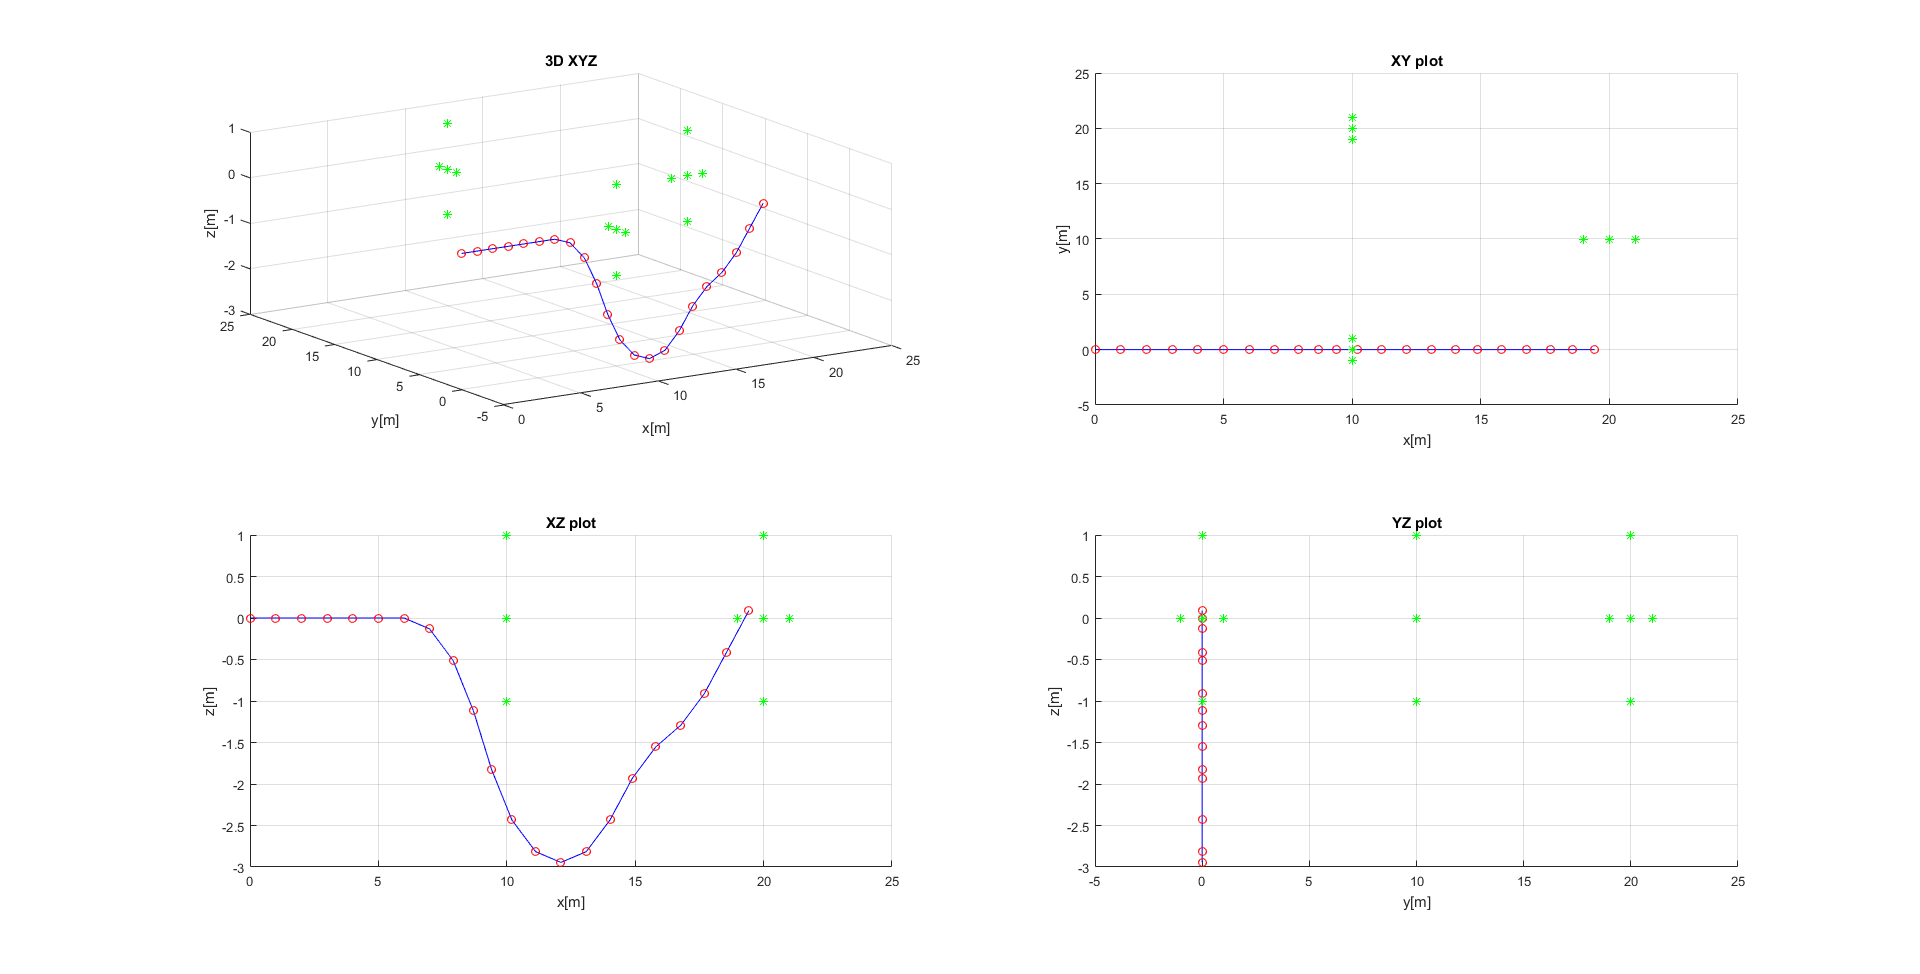
\includegraphics[width=\linewidth]{\FIGDIR/52_First_waypoint_movement.png}
    \caption{First obstacle avoidance at $\mathscr{WP}_1=[20,0,0]^T$.}
    \label{fig:52firstObstacleKnown}
\end{figure}
\noindent Flight between $\mathscr{WP}_S$ to $\mathscr{WP}_1$ was normal and vehicle avoided obstacle choosing bottom path, which is very dangerous in real situation. Real vehicle should choose right,left or top avoidance path in order to minimize collision risks. Decision of rapid exploration algorithm was made, because there is no weight on movement $m_i(t_i)$ in back-stepping calculation process. Trajectory is portrayed in figure \ref{fig:52firstObstacleKnown}. Executed movements during flight from $\mathscr{WP}_S$ to $\mathscr{WP}_1$ have follow values: $B_{\mathscr{MA}}$ = \textit{[$\circledcirc$(6), $\Downarrow$(3), $\circledcirc$(1), $\Uparrow$(5), $\circledcirc$(3), $\Downarrow$(1), $\circledcirc$(1), $\Uparrow$(1)]}. 
\begin{figure}[H]
    \centering
    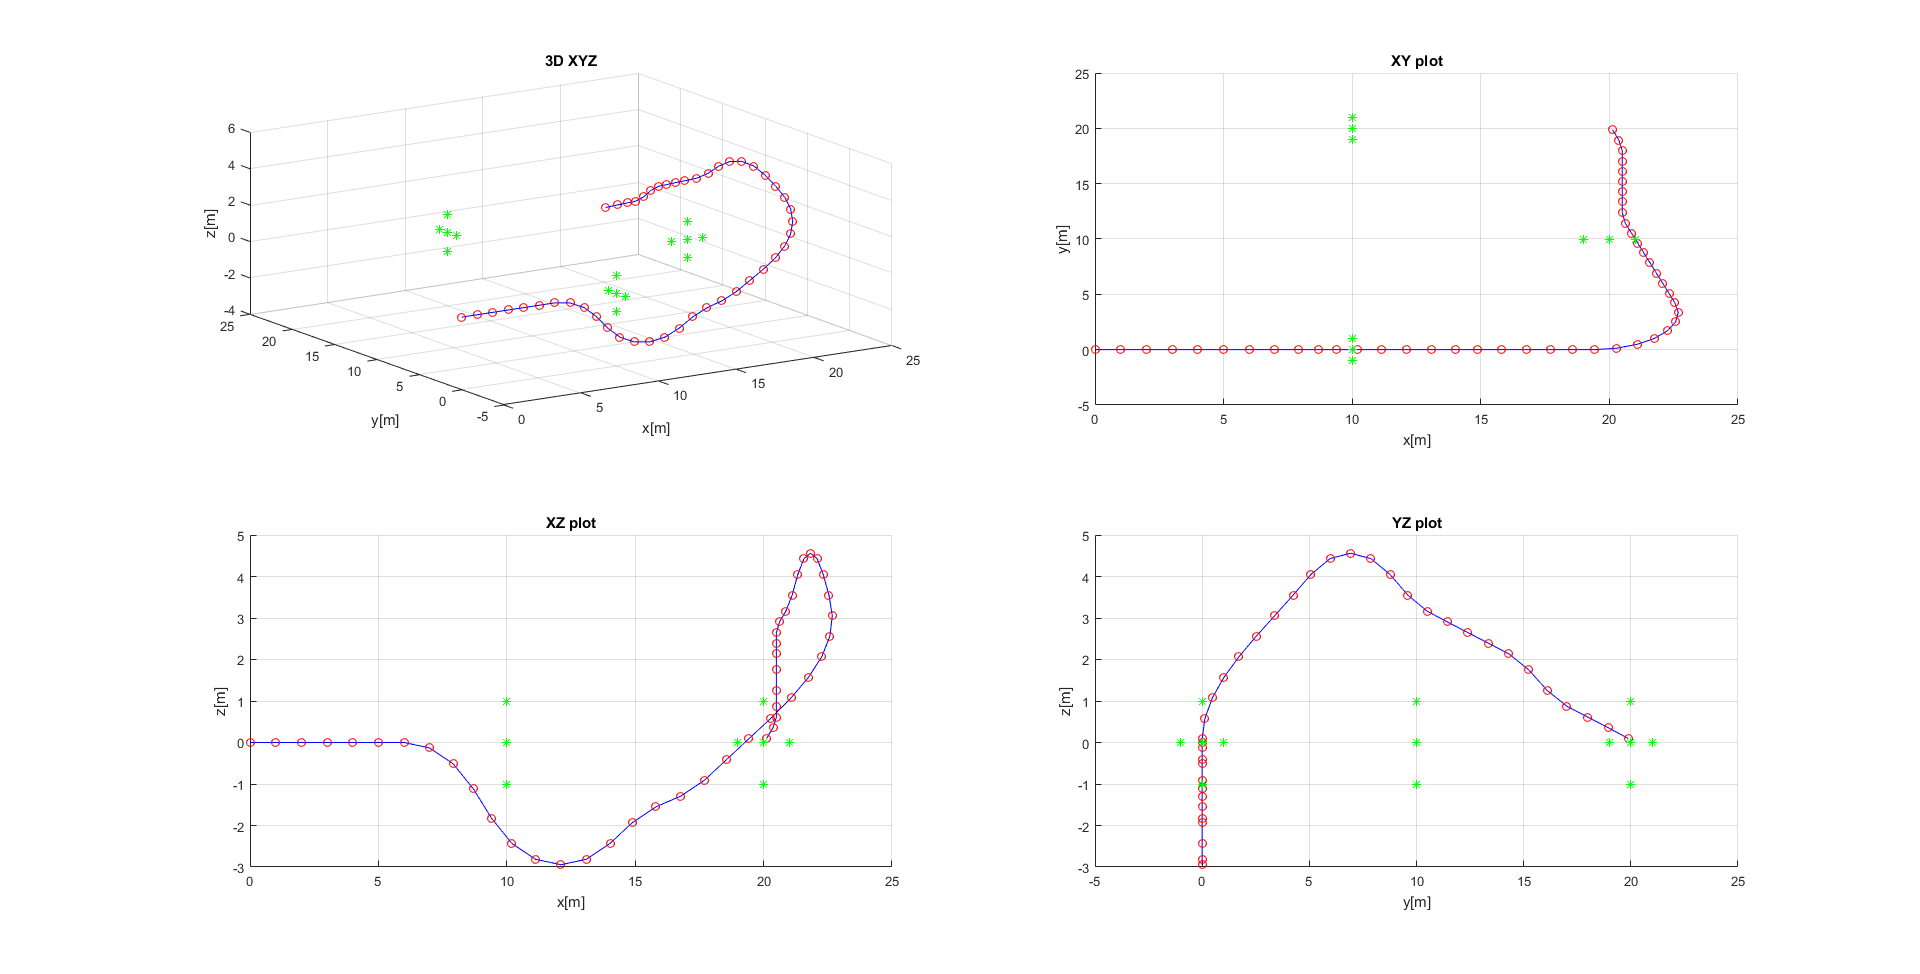
\includegraphics[width=\linewidth]{\FIGDIR/53_Second_waypoint_movement.png}
    \caption{Obstacle avoidance at $\mathscr{WP}_2=[20,20,0]^T$.}
    \label{fig:53secondObstacleKnown}
\end{figure}
\noindent Flight between waypoints $\mathscr{WP}_1$ to $\mathscr{WP}_2$ used top avoidance maneuver, because starting position when obstacle was hindering direct path was a top of obstacle center $o_6=[20,10,0]^T$. Trajectory is portrayed in figure \ref{fig:53secondObstacleKnown}. Executed movements during flight from $\mathscr{WP}_1$ to $\mathscr{WP}_2$ have follow values: $B_{\mathscr{MA}}$ = \textit{[$\Leftarrow$(6), $\circledcirc$(1), $\Downarrow$(1), $\circledcirc$(1), $\Uparrow$(1), $\circledcirc$(1), $\Rightarrow$(1), $\circledcirc$(2), $\Downarrow$(2), $\circledcirc$(1), $\Uparrow$(1), $\circledcirc$(1), $\Leftarrow$(1), $\circledcirc$(1)]}.
\begin{figure}[H]
    \centering
    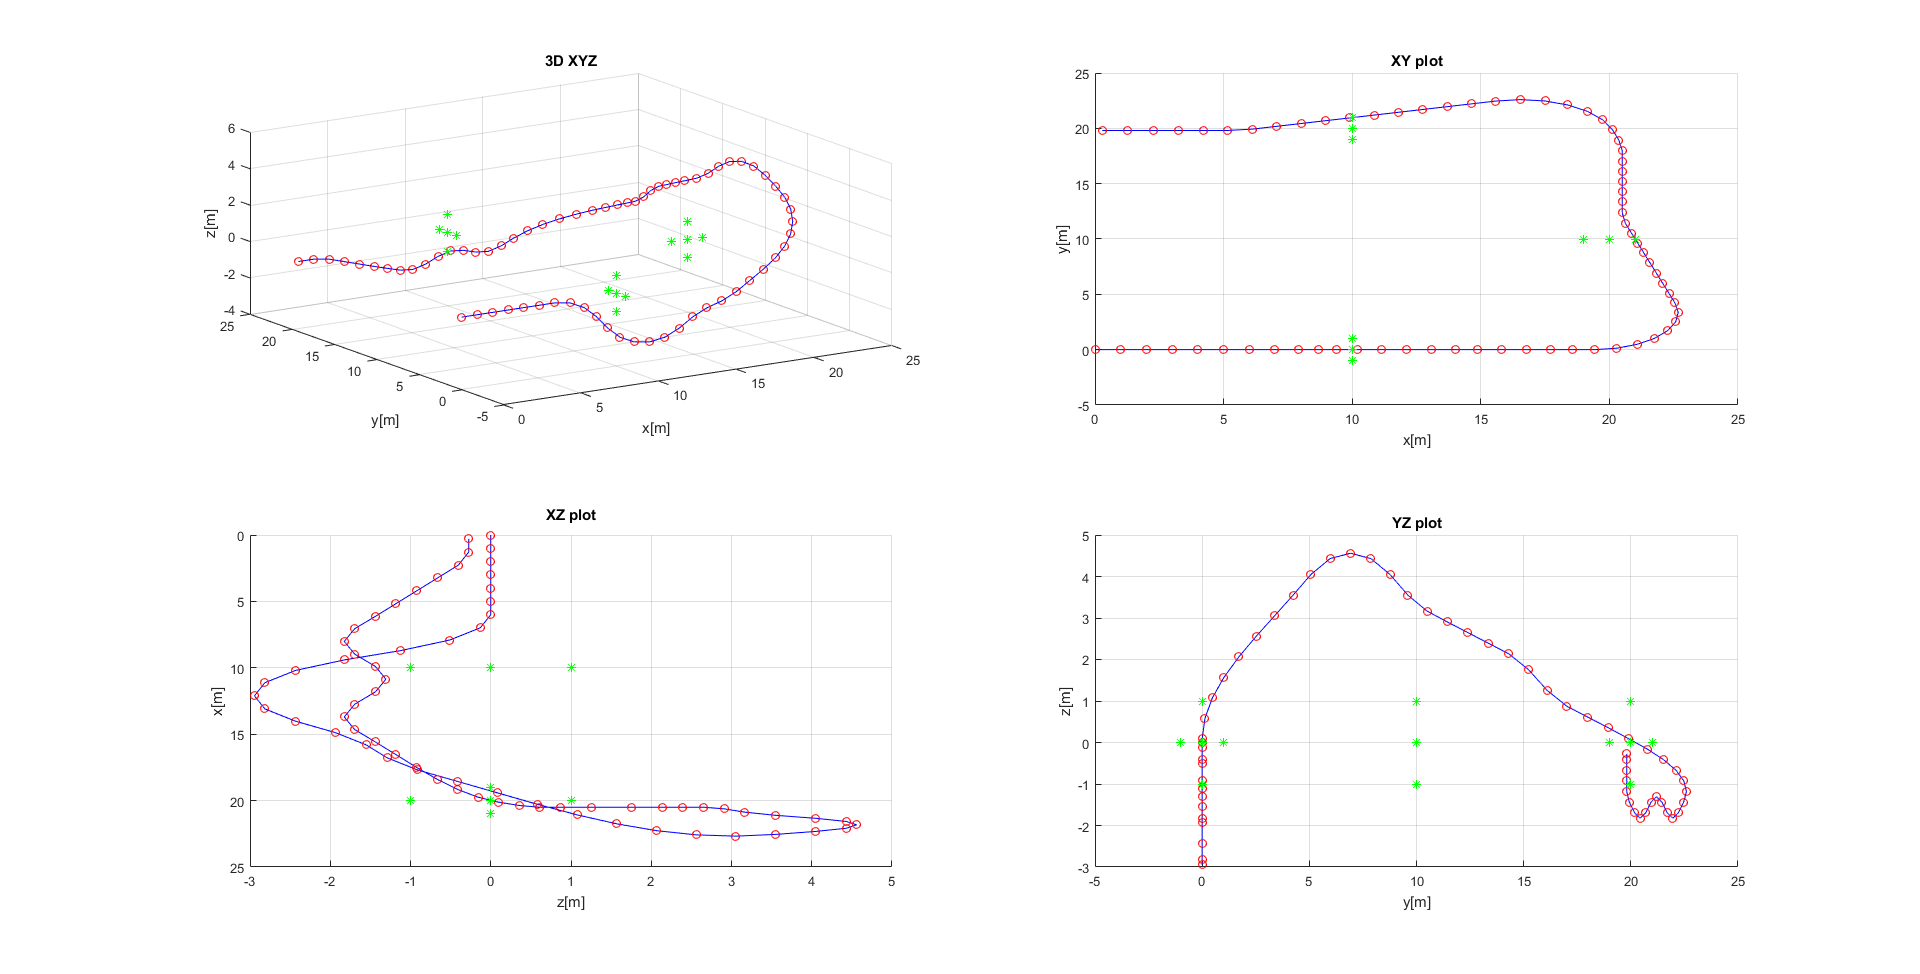
\includegraphics[width=\linewidth]{\FIGDIR/54_Third_waypoint_movement.png}
    \caption{Third obstacle avoidance at $\mathscr{WP}_3=[0,20,0]^T$.}
    \label{fig:54thirdObstacleKnown}
\end{figure}
\noindent Flight between waypoints $\mathscr{WP}_2$ to $\mathscr{WP}_3$ used bottom avoidance maneuver, because starting position when obstacle was hindering direct path was a bottom of obstacle center $o_{11}=[10,20,0]^T$. Trajectory is portrayed in figure \ref{fig:54thirdObstacleKnown}. Executed movements during flight from $\mathscr{WP}_2$ to $\mathscr{WP}_3$ have follow values: $B_{\mathscr{MA}}$ = \textit{[$\Leftarrow$(6), $\circledcirc$(1), $\Uparrow$(2), $\circledcirc$(1), $\Downarrow$(2), $\circledcirc$(1), $\Uparrow$(2), $\circledcirc$(1), $\Rightarrow$(1), $\circledcirc$(2)]}.
\begin{figure}[H]
    \centering
    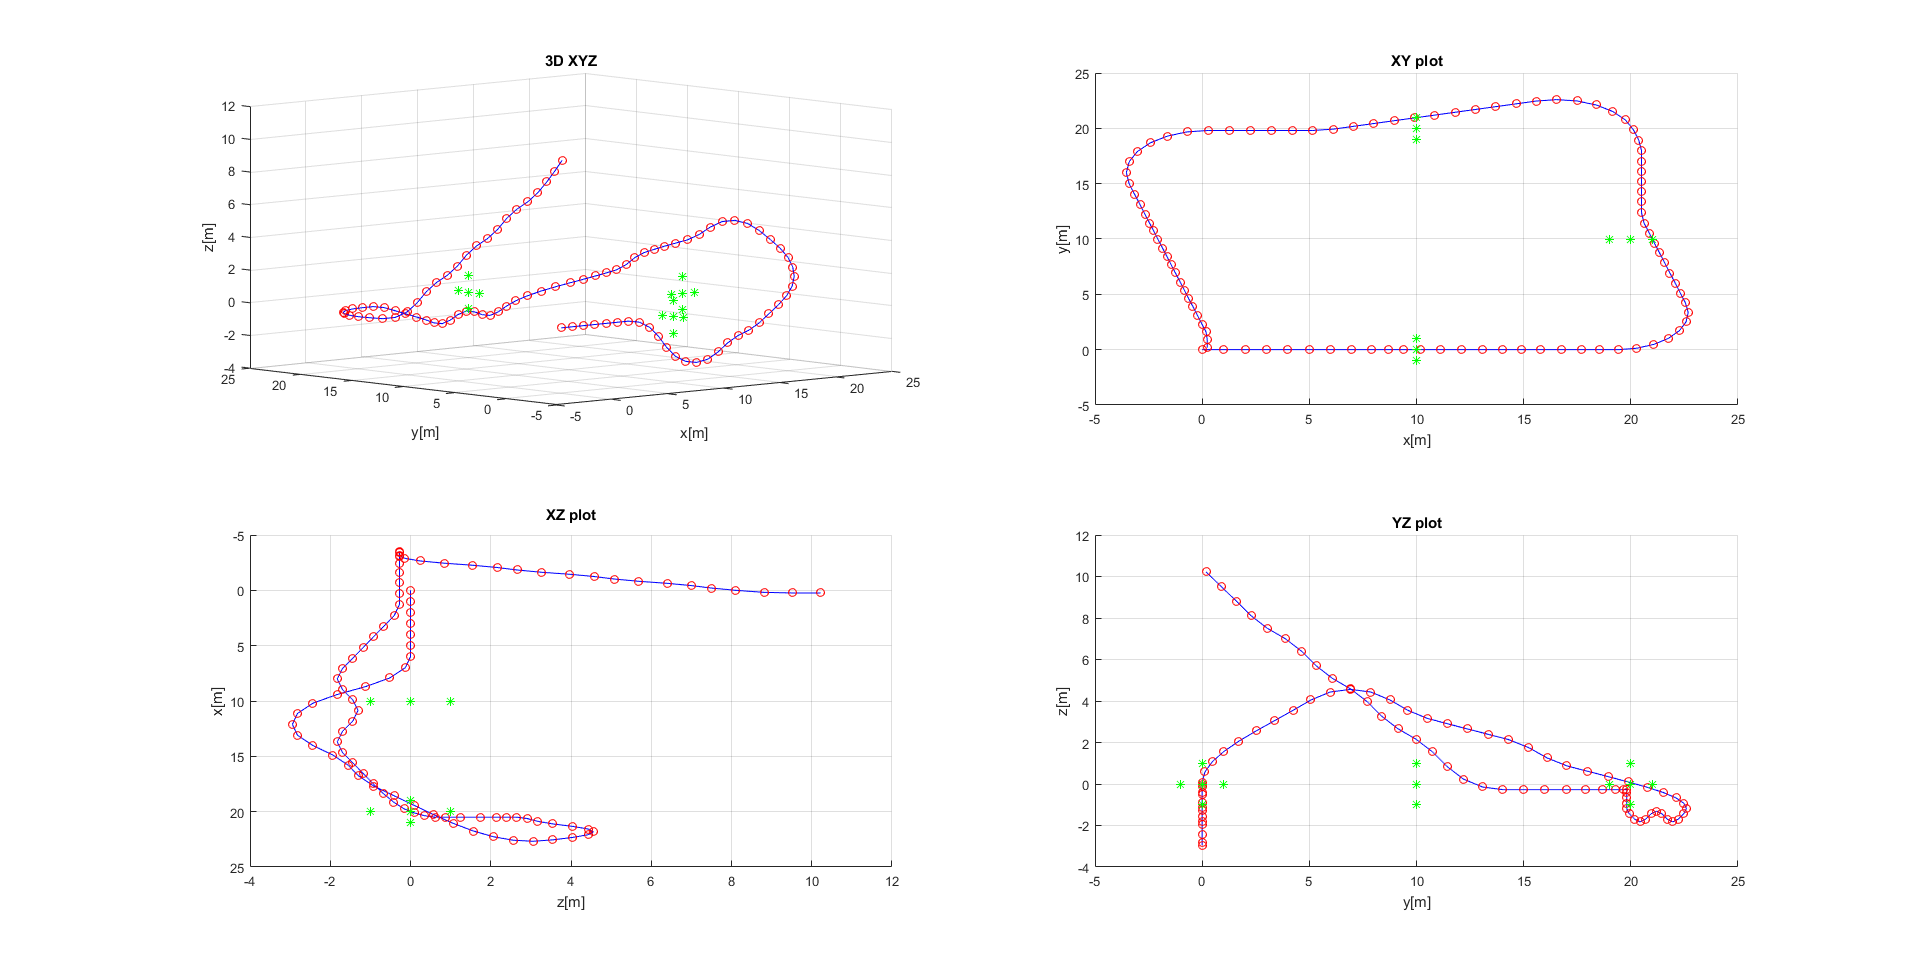
\includegraphics[width=\linewidth]{\FIGDIR/55_Fourth_waypoint_movement.png}
    \caption{Forth waypoint movement at $\mathscr{WP}_4=[0,0,10]^T$.}
    \label{fig:55fourthObstacleknown}
\end{figure}
\noindent Flight between waypoints $\mathscr{WP}_3$ to $\mathscr{WP}_E$ was direct flight between two waypoints until stop condition at $\mathscr{WP}_E$ was triggered. Trajectory is portrayed in figure \ref{fig:55fourthObstacleknown}. Executed movements during flight from $\mathscr{WP}_3$ to $\mathscr{WP}_E$ have follow values: $B_{\mathscr{MA}}$ = \textit{[$\Leftarrow$(7), $\circledcirc$(1), $\Uparrow$(3), $\circledcirc$(1), $\Downarrow$(1), $\circledcirc$(1), $\Uparrow$(1), $\circledcirc$(2), $\Downarrow$(1), $\circledcirc$(1), $\Uparrow$(1), $\circledcirc$(5)]}.
\begin{figure}[H]
    \centering
    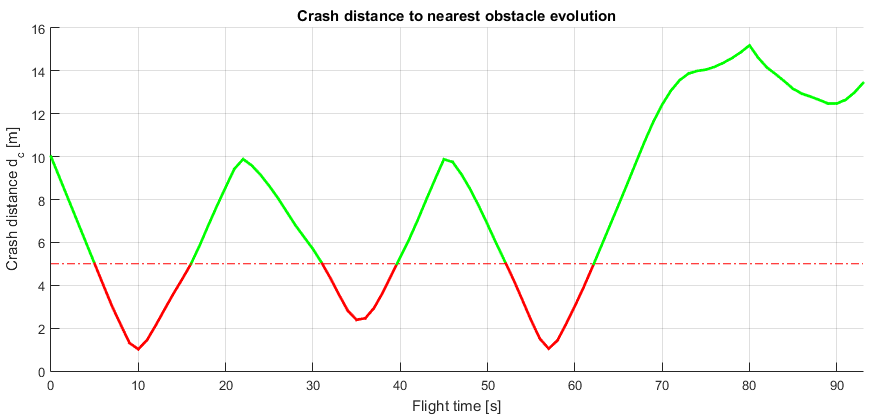
\includegraphics[width=\linewidth]{\FIGDIR/60_Crash_distance_to_nearest_obstacle_evolution_known_world.png}
    \caption{Vehicle crash distance $d_c$ evolution during flight.}
    \label{fig:vehicleCrashDistanceEvolutionKnownWorld}
\end{figure}
\noindent Vehicle crash distance function $d_c$ is vaguely defined as distance to nearest obstacle during time of flight. Crash distance evolution is portrayed in figure \ref{fig:vehicleCrashDistanceEvolutionKnownWorld}. Crash distance $d_c$ was greatest in time of waypoint $\mathscr{WP}_i$ reach, because obstacles $\mathscr{O}$ were positioned in midle between waypoints. Crash distance $d_c$ is divided into two zones:
\begin{enumerate}
    \item \textit{Safe zone} - distance where turn to any direction is possible, this distance is calculated as $2s_m+\mathscr{B}(r)$. In this case was safe distance determined as $5m$.
    \item \textit{Dangerous zone} - distance where turn to any direction is limited. This distance is defined as interval between $B(r)$ and $2s_m+\mathscr{B}(r)$.
\end{enumerate}
Vehicle never breached safety margin $s_m=0.60m$ which is sufficient in this case. Prediction quality is very important factor in predictive control, therefore quantitative measurement for prediction of this system have been introduced (\ref{eq:movementAutomatonPredictionError}). Movement automaton prediction error $e_p$ is based on mean square prediction error (MSE).
\begin{equation}\label{eq:movementAutomatonPredictionError}
    e_p=\sqrt{\sum_{t_i=t_0+i}^{i\in\{1,\dots,n\}} \left (\hat{x}(t_i)-x(t_i)\right)^2}    
\end{equation}

\noindent Movement automaton prediction error compares predicted state $\hat{x}$ and real system state $x$ for each movement execution time $t_i$. Movement execution time in this case was $s_1$ so time $t_i$ was defined as $t_i=t_0+i, i\in\{1,\dots,n\}$, where n is total count of executed movements. Movement automaton prediction error $e_p$ was in this case $e_p\approx 0$.
\begin{figure}[H]
    \centering
    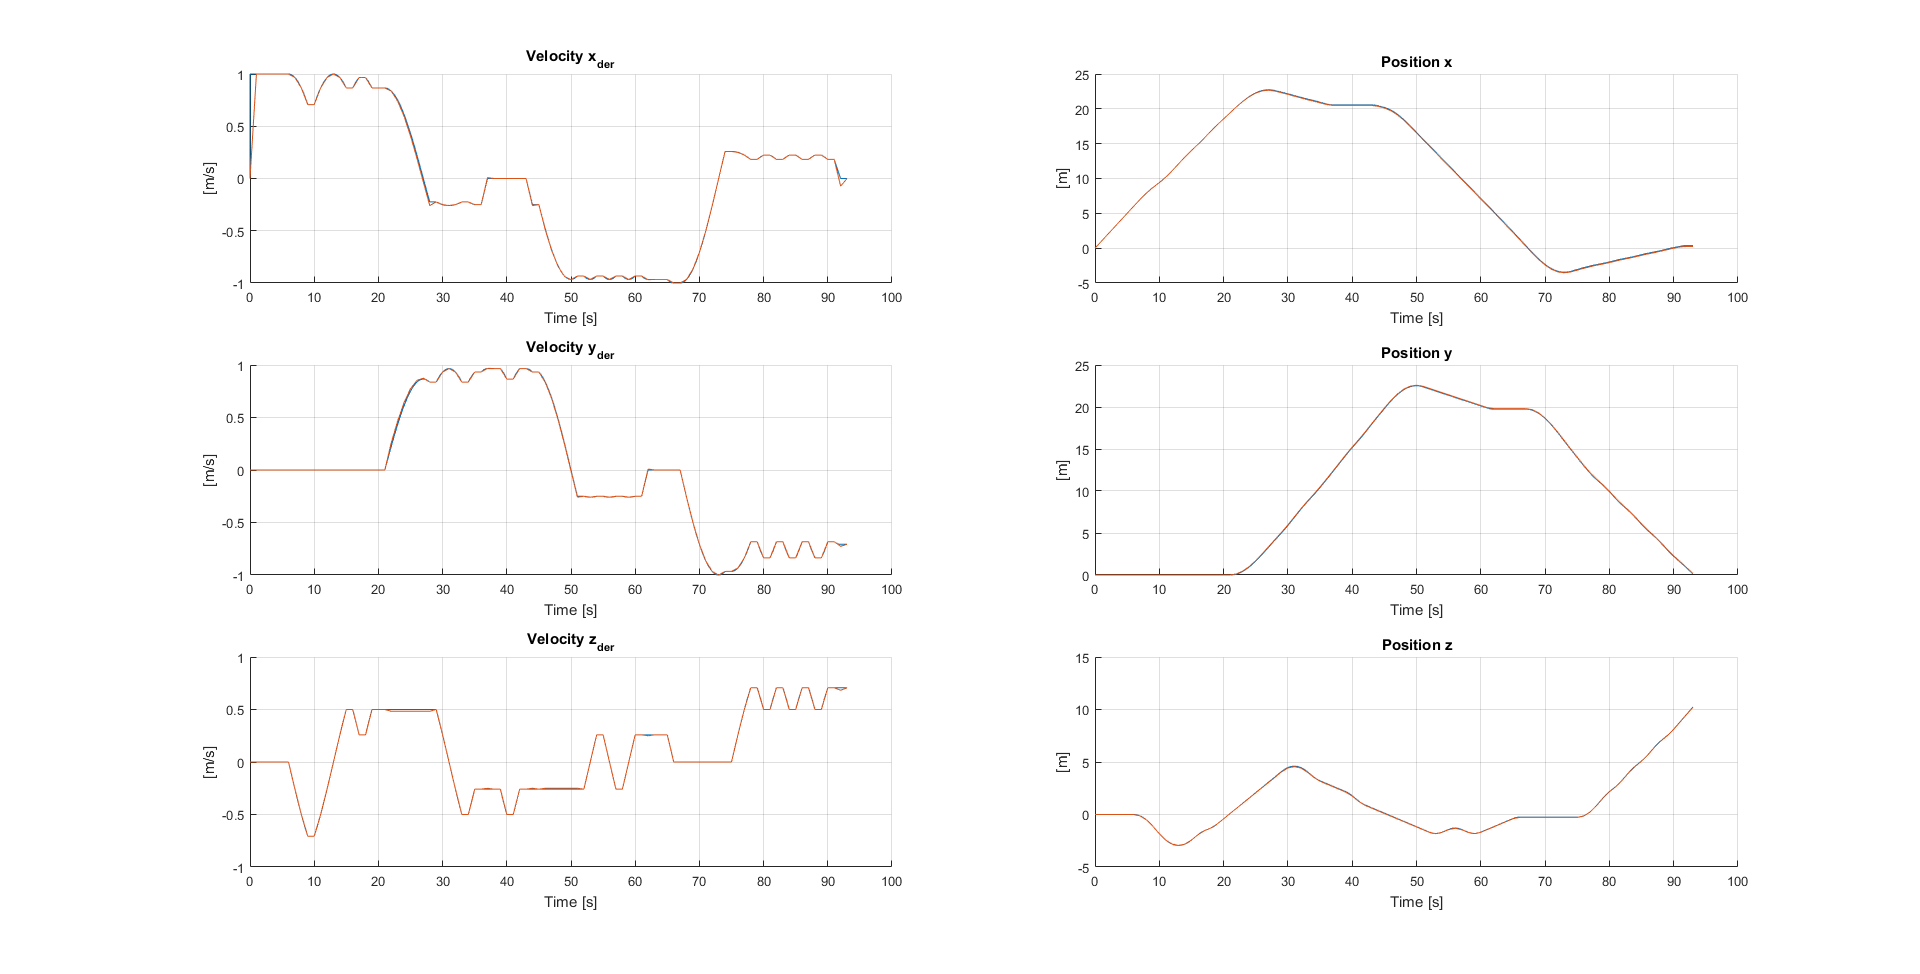
\includegraphics[width=\linewidth]{\FIGDIR/56_Vehicle_position.png}
    \caption{Vehicle position $x,y,z$ and their derivations $\dot{x},\dot{y},\dot{z}$ evolution during flight.}
    \label{fig:vehicleStateKnown1}
\end{figure}
\noindent Vehicle position $x,y,z$ and their derivations $\dot{x},\dot{y},\dot{z}$ and their evolution during flight is portrayed in figure \ref{fig:vehicleStateKnown1}. Brown color is used for predicted model state and blue color is used for real model parameter evolution. Both models are equal, supported by movement automaton prediction error $e_p\approx 0$.
\begin{figure}[H]
    \centering
    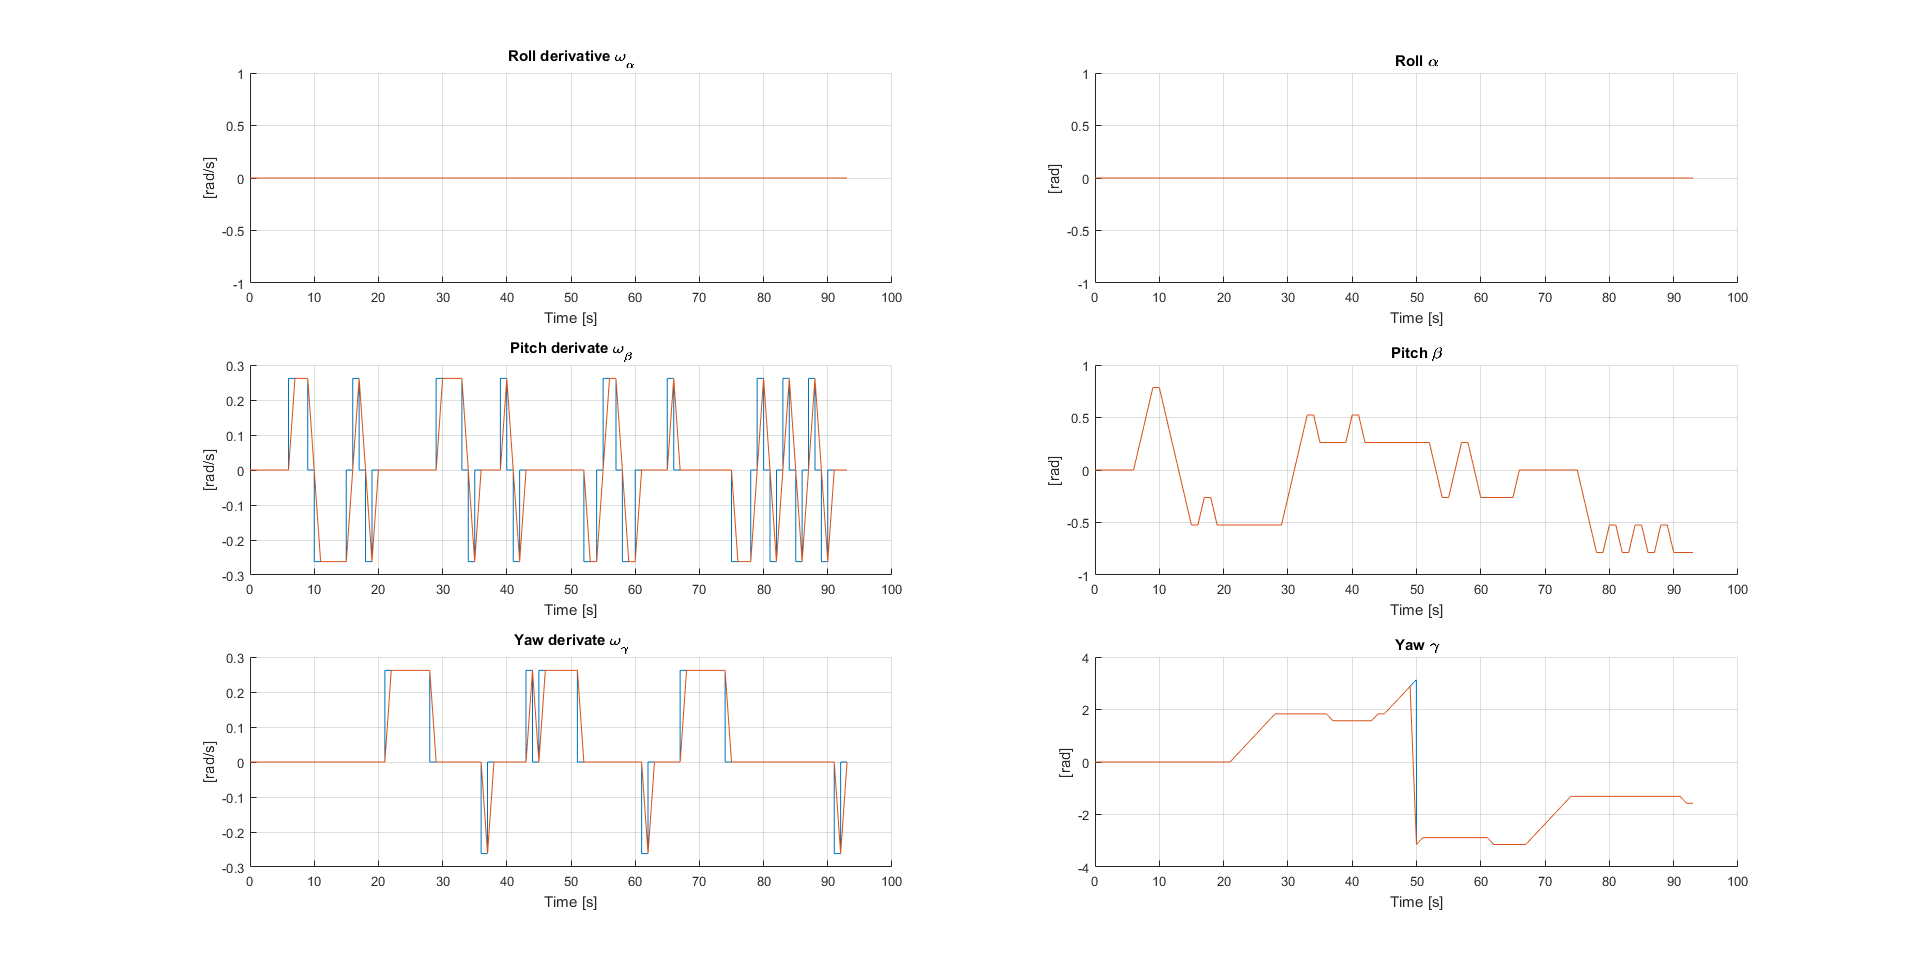
\includegraphics[width=\linewidth]{\FIGDIR/57_Vehicle_angles.png}
    \caption{Vehicle positional angles $\alpha,\beta,\gamma$ and their angular velocities $\omega_\alpha,\omega_\beta,\omega_\gamma$ evolution during flight}
    \label{fig:vehicleStateKnown2}
\end{figure}
\noindent Similar to previous comparison (fig. \ref{fig:vehicleStateKnown1}.) Comparison for vehicle positional angles $\alpha,\beta,\gamma$ and their angular velocities $\omega_\alpha,\omega_\beta,\omega_\gamma$ evolution during flight holds previous assumption (fig. \ref{fig:vehicleStateKnown2}).